\chapter{\texorpdfstring{\MakeUppercase{Introduction}}{Introduction}} \label{chap:intro}

\section{Astrophysical Turbulence Across Scales}

The space between astrophysical objects is far from empty.
Inside galaxy clusters, the intracluster medium (ICM) permeates much of that volume as an X-ray-emitting plasma with characteristic temperature $T \sim 10^8\ \mathrm{K}$ and density $n \sim 10^{-3}\ \mathrm{cm^{-3}}$ \citep[e.g.,][]{fabian_subsonic_1977,sarazin_x-ray_1986}.
In star-forming galaxies, the interstellar medium (ISM) populates the space between stars with a multitude of fluid phases: the warm ionized gas of \ion{H}{2} regions \citep{spitzer_physical_1978,osterbrock_astrophysics_1989}, the neutral medium of atomic hydrogen \citep{field_cosmic-ray_1969,dickey_hi_1990}, and the dense molecular clouds \citep{larson_turbulence_1981}.
Closer to home, the space between us and the Sun is filled with the magnetized solar wind \citep{parker_dynamics_1958,hundhausen_coronal_1972,schwenn_large-scale_1990}.
These environments share one common condition: they are constantly perturbed by physical processes such as mergers, galactic shear, accretion, and feedback from supermassive black holes (SMBHs) and stars.
These perturbations cause the velocity fields in these media to fluctuate unpredictably, producing a feature commonly known as \textit{turbulent flows} \citep{pope_turbulent_2000}.

In a fluid, a turbulent flow develops when the velocity perturbations grow faster than viscosity can damp them.
The ratio between the inertial force, which drives turbulent flows, and the viscous force is characterized by the Reynolds number $Re$.
In general, fluid flows remain laminar at $Re \lesssim 2000$, enter a transition phase over $2000 \lesssim Re \lesssim 4000$, and become turbulent at $Re \gtrsim 4000$ \citep{leishman_introduction_2026}.
Astrophysical flows typically have very large Reynolds numbers, commonly reaching
$Re \sim 10^{10}$ or larger in magnetized astrophysical plasmas
\citep{beresnyak_mhd_2019}. In star-forming molecular clouds, $Re \sim 10^9$ \citep{krumholz_notes_2015}.
Turbulence is thus a ubiquitous phenomenon in the universe.

An astrophysical turbulent flow usually begins with kinetic energy injection into the medium at the \textit{driving scale} $\ell_0$ through supernovae (SNe), mergers, galactic outflows, and other processes, followed by energy transfer to smaller and smaller scales $\ell_0 > \ell_1 > \ell_2 \cdots$, until the kinetic energy is converted into thermal energy via viscous dissipation. 
These turbulent flows manifest as whorls, or eddies, in the fluid (see Figure~\ref{fig:turbulence-spectrum}).
The kinetic energy spectrum of this transfer in an incompressible fluid follows $E(k) \propto k^{-5/3}$ inside the inertial range, assuming homogeneous isotropic turbulence \citep[Kolmogorov turbulence,][]{kolmogorov_local_1941}.
However, many internal and external factors can complicate this picture.

\begin{figure}
    \centering
    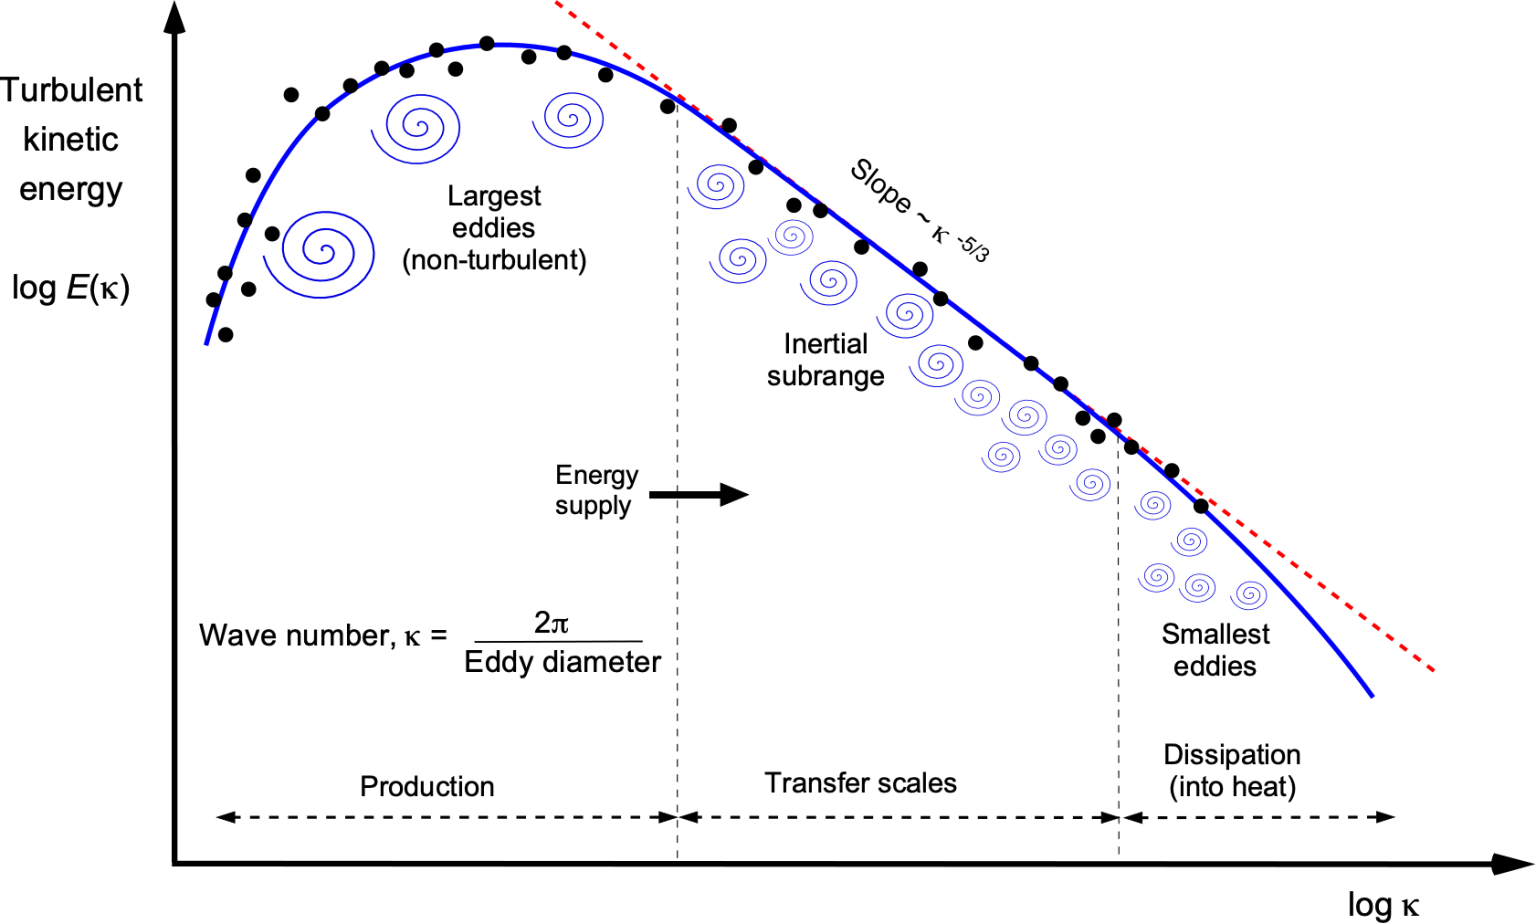
\includegraphics[width=0.9\linewidth]{Intro_img/chapter1_turbulence_spectrum.png}
    \caption[Schematic of a turbulent kinetic energy power spectrum.]{Schematic of a turbulent kinetic energy power spectrum. Reproduced from
    \citet{leishman_introduction_2026}, Chapter 27, Figure 9.}
    \label{fig:turbulence-spectrum}
\end{figure}

\subsection{Effects of compressibility and Mach number on turbulence}

Turbulence can stir a fluid to a characteristic velocity fluctuation, $v_{\rm turb}$. 
Here, the sonic Mach number, $M$, determines the properties of the turbulent flow:
\begin{equation}
    M = \frac{v_{\rm turb}}{c_s},
\end{equation}
where $c_s$\ is the sound speed of the fluid. 
At $M \lesssim 0.3$, pressure waves can smooth out density contrasts and the flow remains close to an incompressible fluid \citep{leishman_introduction_2026}, following the Kolmogorov cascade.
As the flow becomes supersonic ($M \gtrsim 1$), density waves cannot propagate fast enough to smooth out the flow. 
Supersonic turbulence thus introduces shocks that affect the velocity statistics, steepening the kinetic energy spectrum to $E(k) \propto k^{-2}$ \citep[Burgers turbulence,][]{burgers_mathematical_1995,federrath_universality_2013}.

Subsonic, incompressible turbulence is often a good approximation for planetary processes, such as atmospheric disturbances and ocean currents.
Astrophysical environments, however, are often better described by supersonic turbulence.
For example, strong turbulence is seen in multiple galaxy clusters as density contrasts along shock fronts \citep{russell_shock_2012,zhuravleva_turbulent_2014}, while ALMA observations of N159E filamentary CO emission show evidence of compressive turbulence \citep{sharda_first_2022}, and radial velocity fluctuations are seen in multiple \ion{H}{2} regions of the Milky Way and other Local Group galaxies \citep{garcia-vazquez_turbulence_2023}.

\subsection{Effects of magnetic fields and intermittency on turbulence}

Beyond compressibility, astrophysical turbulence can also be shaped by additional physics, especially magnetic forces.
In astrophysical plasmas, magnetic fields are dynamically coupled to the fluid through the Lorentz force, so turbulence not only transfers kinetic energy across scales, but also contributes to twisting magnetic field lines, which in turn converts kinetic energy to magnetic energy \citep[e.g.,][]{biskamp_magnetohydrodynamic_2003, beresnyak_mhd_2019}.
In magnetohydrodynamic (MHD) turbulence, two numbers control the characteristics of the flow: the Alfv\'en Mach number, $M_{\rm A}$, and the plasma $\beta$:
\begin{equation}
    M_{\rm A} = \frac{v_{\rm turb}}{v_{\rm A}},
\end{equation}
where $v_{\rm A} = B/\sqrt{4\pi \rho}$\ is the Alfv\'en speed.
The Alfv\'en Mach number measures whether the magnetic field strongly guides the turbulent cascade ($M_{\rm A} < 1$) or if turbulent motions can twist the field more easily ($M_{\rm A} > 1$).
\begin{equation}
    \beta = \frac{P_{\rm gas}}{P_{\rm mag}},
\end{equation}
which is the ratio between thermal pressure and magnetic pressure.
The plasma $\beta$\ parameter indicates how strongly the magnetic field affects the properties of turbulence in a fluid.

Importantly, magnetic fields introduce \textit{anisotropy} to a turbulent velocity field, breaking the isotropic assumption of Kolmogorov turbulence. 
In the strong MHD regime, energy transfers more efficiently perpendicular to the local magnetic field than parallel to it, producing elongated eddies, while the perpendicular kinetic energy spectrum remains Kolmogorov-like, $E(k_{\perp}) \propto k_{\perp}^{-5/3}$ \citep{goldreich_toward_1995}.
For example, in situ measurements of the fast solar wind show anisotropic magnetic-field fluctuations with different spectral scalings parallel and perpendicular to the local field \citep{wicks_power_2010}, while Galactic \ion{H}{1} observations reveal long, magnetically aligned fibers that trace the projected interstellar magnetic field \citep{clark_magnetically_2014}.

Another important characteristic of MHD turbulence, especially at small scales, is intermittency. 
Intermittency is the tendency of a turbulent flow not to follow a statistically uniform distribution, but instead to become increasingly sparse in time or space with decreasing scale size \citep{biskamp_magnetohydrodynamic_2003}.
In magnetized plasma turbulence, intermittency manifests as current sheets; this manifestation is discussed in more detail in Chapter~\ref{chap:ml}.
Figure~\ref{fig:turbulence-regimes} illustrates these characteristics across four examples of astrophysical turbulence modified by strong shocks \citep{russell_shock_2012}, supersonic driving \citep{federrath_universality_2013}, \ion{H}{2} ionization \citep{medina_turbulence_2014}, and intermittency \citep{dong_reconnection-driven_2022}.

\begin{figure}
    \centering
    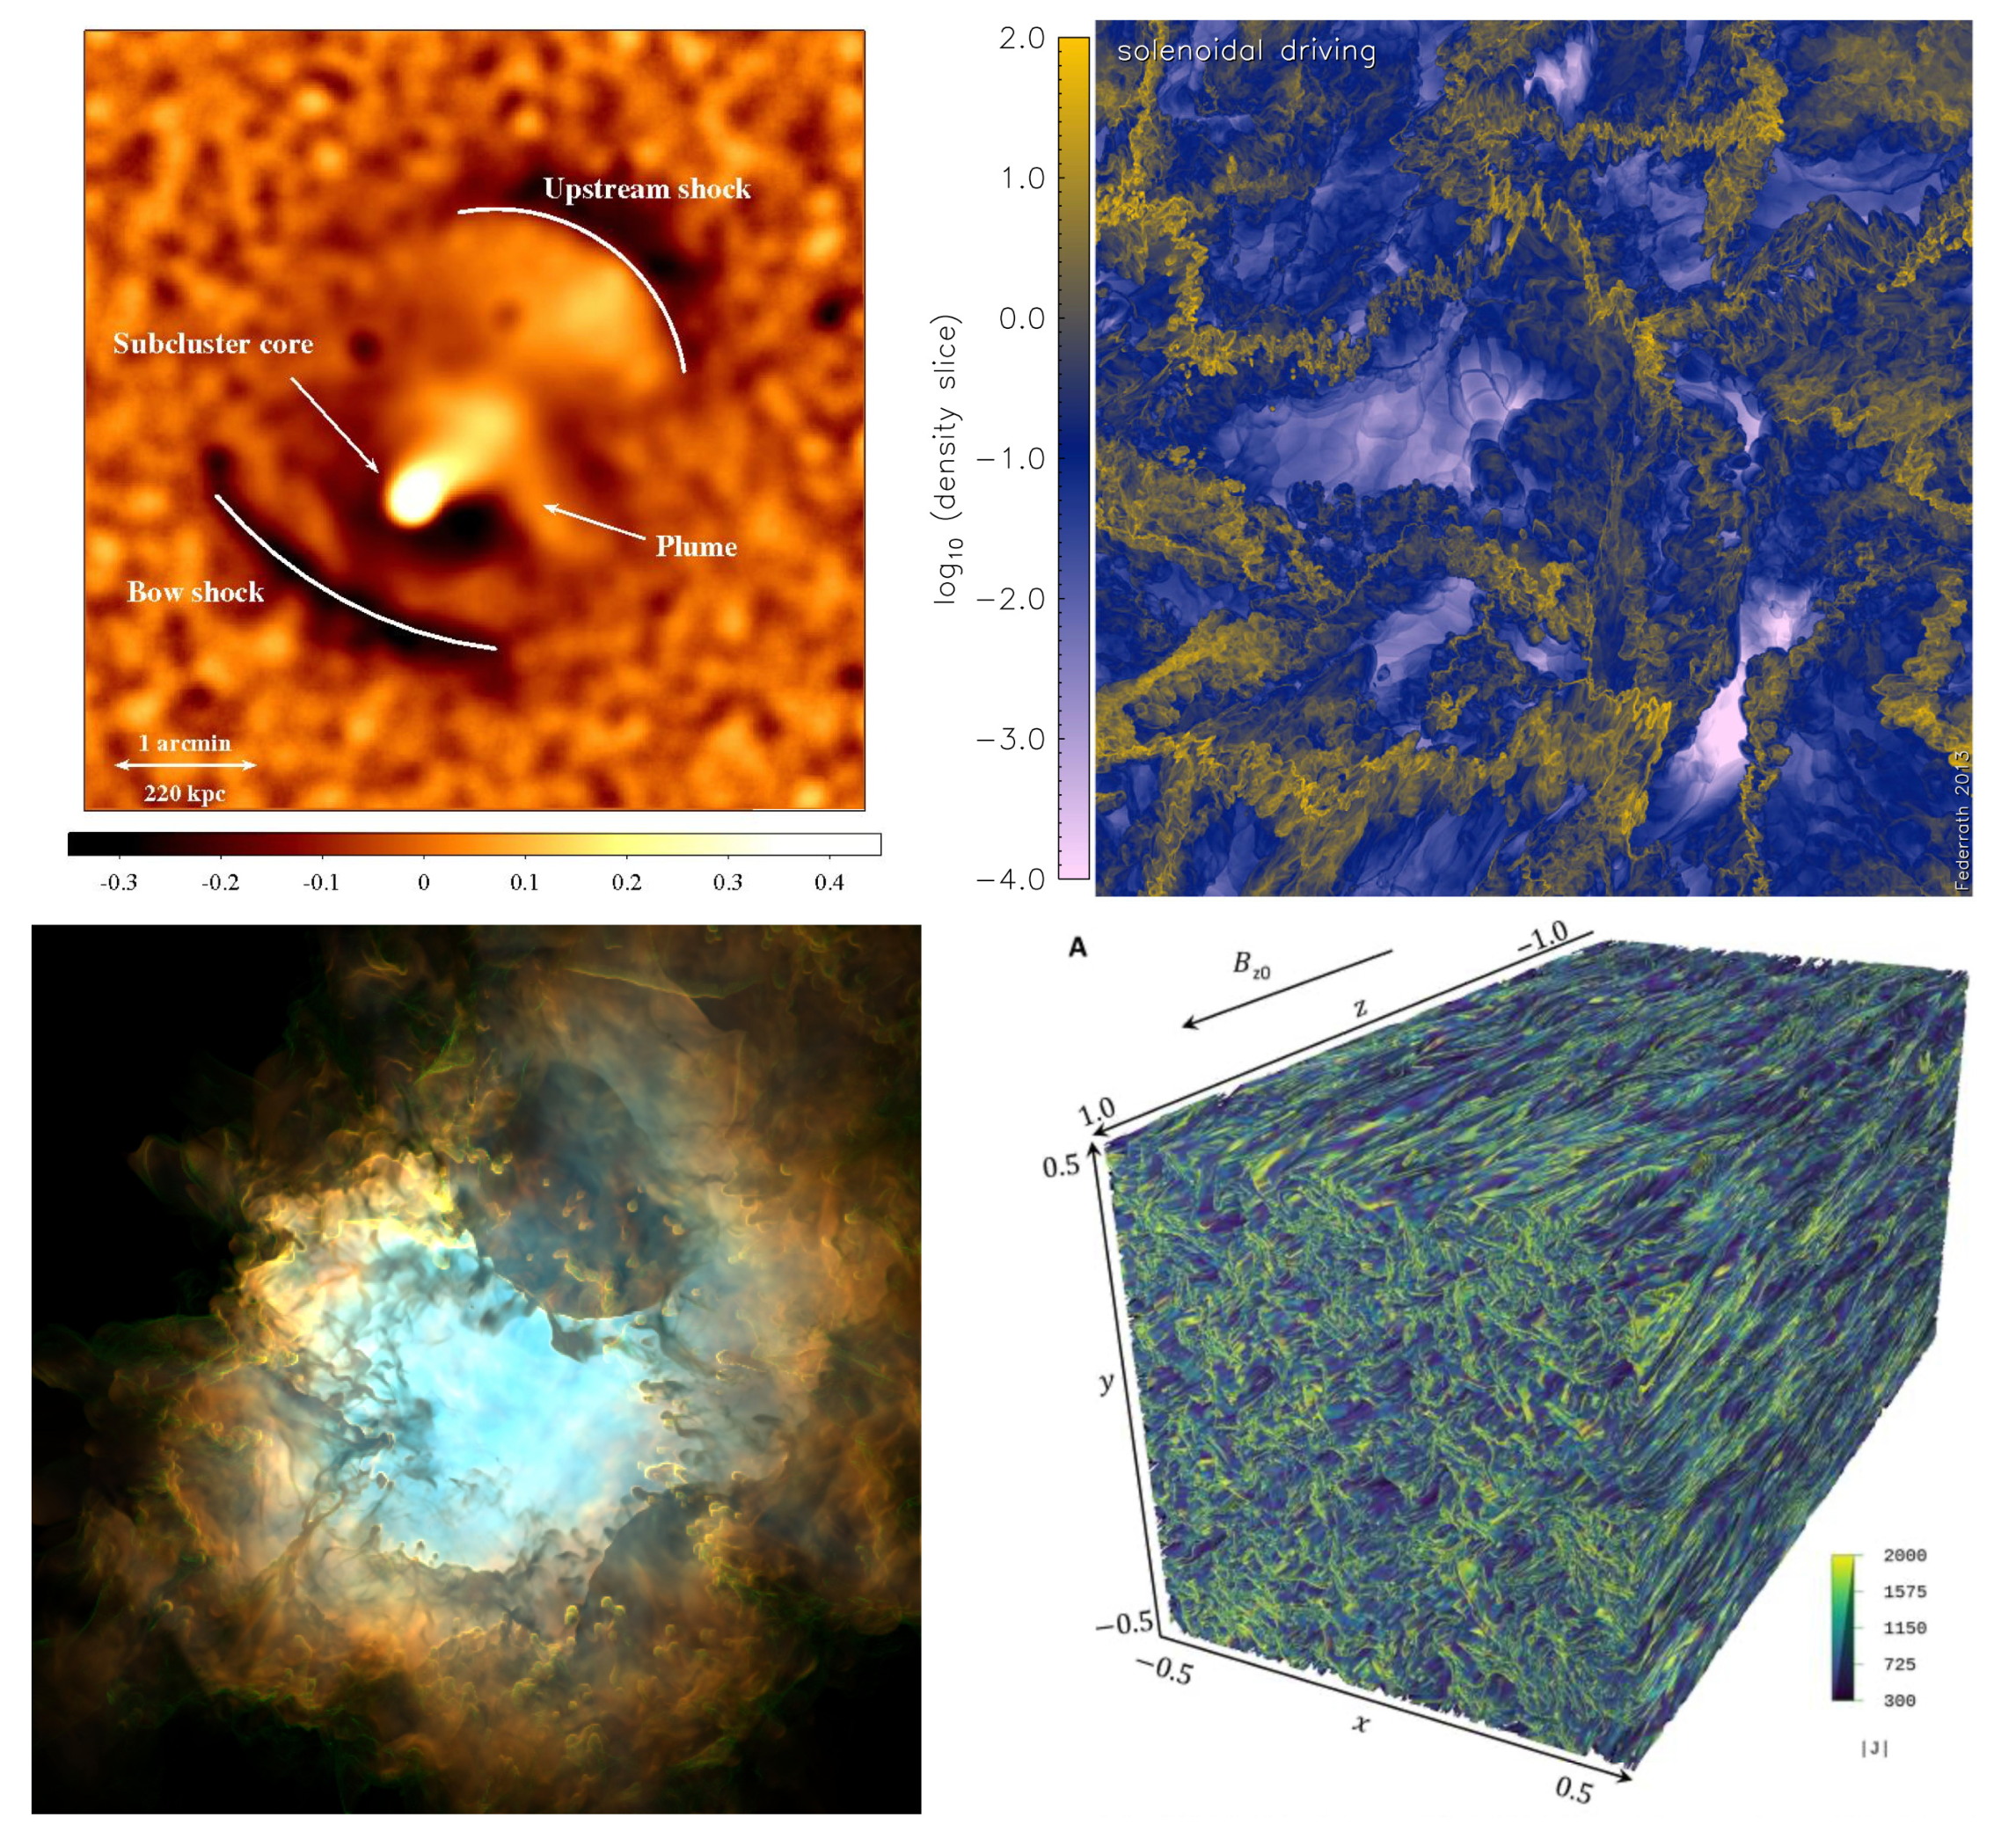
\includegraphics[width=\linewidth]{Intro_img/chapter1_turbulence_regimes.pdf}
    \caption{Representative examples of astrophysical turbulence beyond the Kolmogorov model. Top left: shock fronts observed in galaxy cluster Abell 2146, caused by a merger. Adapted from \citet{russell_shock_2012}. Top right: a slice of a solenoidally driven turbulence simulation, with structure similar to that found in the ISM\@. Adapted from \citet{federrath_universality_2013}. Bottom left: simulated projected image of an evolving \ion{H}{2} region in a turbulent molecular cloud. Adapted from \citet{medina_turbulence_2014}. Bottom right: volume rendering of current density in fully developed MHD turbulence. Adapted from \citet{dong_reconnection-driven_2022}.}
    \label{fig:turbulence-regimes}
\end{figure}

\section{The Three Regimes of Astrophysical Turbulence in This Dissertation}

\begin{table}[t]
\centering
\caption{Three regimes of turbulence and diagnostic tools studied in this dissertation.}
\label{tab:intro-regimes}
\renewcommand{\arraystretch}{1.25}
\begin{tabular}{@{}>{\raggedright\arraybackslash}p{0.24\textwidth}>{\raggedright\arraybackslash}p{0.68\textwidth}@{}}
\toprule
Regime & Physical setting and diagnostic approach \\
\midrule
Active galactic nucleus (AGN) atmospheres &
Scale: $10^4$--$10^6\ \mathrm{pc}$\newline
Main drivers: SMBH jet feedback in low-accretion-rate systems\newline
Main limitation: unresolved accretion physics\newline
Diagnostic: hydrodynamic multi-scale simulations \\
ISM and molecular clouds &
Scale: $10^0$--$10^4\ \mathrm{pc}$\newline
Main drivers: stellar outflows, SNe, and galactic shear\newline
Main limitation: projection and tracer bias\newline
Diagnostic: velocity statistics from young stars \\
Relativistic plasma &
Scale: $10^{-4}$--$10^{-1}\ \mathrm{pc}$\newline
Main driver: magnetic-field fluctuations\newline
Main limitation: inefficient identification of intermittent structures in large datasets\newline
Diagnostic: machine-learning segmentation \\
\bottomrule
\end{tabular}
\end{table}

Astrophysical turbulence plays an important role in shaping gas morphology across vast spatial scales.
This dissertation focuses on three representative regimes across that large dynamical range (see Table~\ref{tab:intro-regimes} for a summary):
\begin{enumerate}
    \item $10\ \mathrm{kpc} \lesssim \ell \lesssim 1\ \mathrm{Mpc}$: in the circumgalactic medium (CGM) at the outskirts of galaxies and in the ICM, SMBH feedback injects vast amounts of energy ($\dot{E} \approx 10^{42}\text{--}10^{45}\ \mathrm{erg\ s^{-1}}$) into the surrounding medium, helping to balance the overall radiative cooling of the X-ray-emitting atmosphere \citep{fabian_cooling_1994}. In low-luminosity systems such as M87, this feedback is dominated by relativistic jets \citep{fabian_observational_2012,li_direct_2020}, while high-accretion-rate systems can also drive accretion-disk winds and radiative outflows \citep[][]{murray_accretion_1995}.
    \item $1\ \mathrm{pc} \lesssim \ell \lesssim 10\ \mathrm{kpc}$: inside the ISM, cold and dense molecular clouds collapse under self-gravity to form stars.
    Various stellar processes such as winds and SNe drive turbulence on pc scales and regulate the star formation process \citep[][]{mac_low_control_2004,mckee_theory_2007,hennebelle_turbulent_2012}.
    Galactic shear and other large-scale processes also drive turbulence in this regime \citep[e.g.,][]{piontek_models_2007,forbes_gas_2023}.
    \item $10^{-4}\ \mathrm{pc} \lesssim \ell \lesssim 0.1\ \mathrm{pc}$: in extremely high-energy environments near rapidly accreting neutron stars and black holes, at scales comparable to the object's gravitational radius, the flows are accompanied by strong magnetic-field fluctuations \citep{biskamp_magnetohydrodynamic_2003, beresnyak_mhd_2019}.
    The non-linear interactions between the magnetic field and local plasma produce violent energy dissipation events observed in gamma-ray bursts \citep[e.g.,][]{beniamini_prompt_2017,lazarian_gamma-ray_2019}.
\end{enumerate}

\section{Limitations of Existing Techniques in Measuring Turbulence}

Astrophysical turbulence is notoriously difficult to measure. 
Turbulence is multi-dimensional and time-dependent, yet the tools we possess to probe it predominantly offer an incomplete picture of the flow.
Spectral observations can only probe the line-of-sight (LOS) velocity and the plane-of-the-sky position, leaving unresolved projection uncertainties.
Spatially, turbulence can span many orders of magnitude (see the previous section for examples of the length scales involved), but current instruments are resolution-limited and can only probe parts of a turbulent cascade \citep[e.g.,][]{hitomi_collaboration_atmospheric_2018,churazov_x-ray_2012}.
Observations of turbulence are also limited by the choice of tracer, since turbulence manifests differently in different phases of gas. 
For example, the ISM contains both cold molecular gas ($T \approx 10^2\ \mathrm{K}$) and warm ionized gas ($T \approx 10^4\ \mathrm{K}$). 
Studies have suggested that most of the kinetic energy injected by SNe is deposited into low-density regions of the ISM \citep[see, e.g.,][]{kim_momentum_2015,padoan_supernova_2016}, driving significant turbulence in the warm ionized gas while leaving the molecular phase comparatively less perturbed.
Therefore, no single observational campaign can recover the full velocity field and energy cascade of a turbulent system.

The problem becomes even more pronounced in time.
The turbulent timescales in the molecular ISM are on the order of $10^6$--$10^7$ years \citep{sun_molecular_2022}, and ICM turbulent timescales are even longer, $\sim 10^8$--$10^9$ years \citep{hitomi_collaboration_atmospheric_2018}. 
Meanwhile, the longest survey conducted to study how turbulence evolves in the solar wind has only been collecting data for the past $\sim 30$\ years \citep{wilson_quarter_2021}.
In essence, observations only provide snapshots of complex environments where the turbulent cascade and its driving processes coexist and are difficult to untangle.

Since the turn of the century, advances in numerical methods and computational capabilities have enabled a different kind of turbulence modeling.
Currently, two numerical treatments are commonly used to model astrophysical turbulence.
At the galaxy scale, MHD simulations discretize fluid variables onto grid cells, making it possible to follow gas, magnetic fields, gravity, cooling, and feedback over large volumes \citep[e.g.,][]{somerville_physical_2015,beresnyak_mhd_2019}.
In systems where Lorentz-force coupling is important, such as magnetic reconnection near compact objects, relativistic jets, or pulsar winds, particle-in-cell simulations are often the preferred treatment because they evolve charged particles and electromagnetic fields together \citep[e.g.,][]{zweibel_magnetic_2009,kagan_relativistic_2015}.
These simulations give us access to time evolution of turbulence that observations cannot provide, but other challenges remain.
Galaxy simulations cannot resolve dissipation scales, while particle-in-cell simulations resolve kinetic physics only in domains far smaller than the astrophysical systems they represent.
Running such calculations is also expensive, so modern simulations remain approximations of real environments rather than complete reconstructions.
To understand the full picture of turbulence from global driving to local dissipation, next-generation multi-scale methods are needed to bridge this gap.

\section{Introducing the Next Generation of Diagnostic Tools for Turbulent Systems}

This dissertation brings together six years of research on the nature of turbulence in the three physical regimes introduced above.
Specifically, I developed and applied \textit{diagnostic tools}: statistical, machine-learning, and simulation frameworks that turn incomplete data into physical constraints on a turbulent system.
The first diagnostic tool uses young stars as tracers of the turbulent velocity field in their natal molecular clouds.
In Chapter~\ref{chap:stars}, I introduce this method through two first-author studies: a proof-of-concept application to the Orion Complex, where stellar kinematics reveal a signature of the turbulent cascade \citep{ha_measuring_2021}, and a broader comparison across Ophiuchus, Perseus, and Taurus, where stellar velocity statistics are benchmarked against gas kinematic measurements \citep{ha_turbulence_2022}.
Together, these studies established the conditions under which young stars can preserve information about molecular-cloud turbulence, how subsequent dynamical evolution contaminates this information, and how multi-tracer measurements can distinguish between different drivers of turbulence in star-forming environments.

The second diagnostic tool applies machine learning to intermittent structures in relativistic plasma turbulence.
In Chapter~\ref{chap:ml}, I introduce \awesom, a theory-agnostic clustering package based on self-organizing maps and ensemble learning that I developed to identify complex structures in large simulation datasets \citep{ha_awesom_2025}.
I then apply \awesom\ to three-dimensional plasma simulations, showing that machine-learning methods can identify current sheets with high accuracy and separate them into distinct ``single current sheet'' and ``double current sheet'' morphologies \citep{ha_machine_2025}.
These morphologies form under different physical conditions and may dissipate energy at different rates, making them important targets for future subgrid treatments of plasma turbulence.

The third diagnostic tool uses hydrodynamic simulations to study turbulent multiphase accretion flows onto SMBHs.
In Chapter~\ref{chap:sim}, I describe a suite of simulations from an upcoming first-author study, \citet{ha_galaxy-_2026}, that probes low-luminosity AGN accretion, the limits of the Bondi accretion model, and resolution effects that shape the morphology of cool gas.
This simulation-based diagnostic complements the statistical and machine-learning tools developed in the previous chapters by using controlled numerical experiments to connect unresolved accretion physics with observable multiphase structure.

\section{Related Works}

As a graduate researcher, I had the pleasure of contributing to several research projects that concluded in peer-reviewed publications. 
Although these publications are not highlighted in the main body of this dissertation, they coincide with the overarching goal of my doctoral work: to develop statistical and machine-learning tools that advance our ability to measure astrophysical turbulence and that can be reused and extended by future studies. 

\subsection{As Contributing Author}

I was the third author of \citet{velguth_probing_2025}, which extends the analyses from my early works \citep{ha_measuring_2021, ha_turbulence_2022}.
It is a natural generalization of the young-star turbulence framework: rather than treating the stellar velocity structure function (VSF) only as a measurement of inherited molecular-cloud turbulence, we used the same diagnostic to ask how that initial turbulent imprint is modified by subsequent dynamical evolution and environmental effects (e.g., from gravity, SNe, Galactic shear, and magnetic fields). 
I was directly involved in mentoring the first author, a post-baccalaureate fellow, during the early months of the project, helping to frame the scientific question, interpret the VSF results, and connect the analysis to the methodology developed in Chapter~\ref{chap:stars}.

I was also the third author of \citet{reinheimer_black_2025}, which introduces machine-learning regression to model SMBH--host galaxy relationships. 
Previously, these relationships were modeled by linear fits to a single feature ($\sigma$, $M_{\star}$, $M_{\rm halo}$), which introduced large uncertainties at low SMBH mass. 
We found that several machine-learning regression algorithms, such as XGBoost and multi-layer perceptrons, could provide better predictions of the SMBH mass throughout the mass range, suggesting that these algorithms are better at handling the intrinsic non-linearity of astrophysical systems.
Furthermore, combining multiple host-galaxy properties produced more accurate SMBH mass predictions than any individual one-dimensional scaling relation.
This work, together with the algorithm that I detail in Chapter~\ref{chap:ml}, highlights how machine-learning methods can evolve beyond curve fitting or classification alone to reveal physically meaningful structure in large, complex astrophysical datasets.

\subsection{As First Author}

I was the first author on one other project during this period, which addressed a related problem in observational quasar accretion physics. 
In \citet{ha_shedding_2023}, I studied weak emission-line quasars (WLQs), a subset of type 1 quasars with unusually weak rest-frame ultraviolet (UV) emission lines, and investigated how their emission-line properties connect to black-hole accretion rates. 
By comparing WLQs with ordinary quasars in the \ion{C}{4} equivalent-width--blueshift parameter space, I showed that traditional broad-line-region size--luminosity empirical relations can overestimate WLQ black-hole masses by up to an order of magnitude without a correction to the optical \ion{Fe}{2} emission.
I then used the corrected Eddington luminosity ratios (a proxy of black hole accretion rates) to find a significant correlation with a multi-dimensional \ion{C}{4} spectral feature across both WLQs and ordinary quasars.
From this result, we concluded that WLQs are not outliers compared to other type 1 quasars, but instead are preferentially situated at the tail of a multi-dimensional UV distribution without being statistically out of distribution. 
% Although this work falls outside the main turbulence-focused structure of the dissertation, it reflects the same broader interest in using imperfect observational signals to infer the physical state of accreting SMBHs, a topic I address in Chapter~\ref{chap:sim}.
Although this work falls outside the main turbulence-focused structure of the dissertation, it addresses a similar question about the physical state of accreting SMBHs, which I revisit through simulation in Chapter~\ref{chap:sim}.

\section{Dissertation Outline}

The following chapters detail three research projects I have led during my doctoral work, each focused on a different diagnostic approach to astrophysical turbulence. In Chapter~\ref{chap:stars}, I present young-star velocity statistics as a tracer of turbulence in star-forming molecular clouds. In Chapter~\ref{chap:ml}, I develop and apply machine-learning methods to identify intermittent current sheets in relativistic plasma simulations. In Chapter~\ref{chap:sim}, I use hydrodynamic simulations to study turbulent multiphase accretion flows onto SMBHs. Finally, Chapter~\ref{chap:summary} summarizes the dissertation and outlines future work.
